\documentclass[12pt,a4paper]{article}

% Margins.
\setlength{\oddsidemargin}{0in}
\setlength{\evensidemargin}{0in}
\setlength{\headheight}{12pt}
\setlength{\headsep}{42pt}
\setlength{\topmargin}{-54pt}
\setlength{\textwidth}{6.5in}
\setlength{\textheight}{10in}

\usepackage{amsmath}
\usepackage{float}
\usepackage{graphicx}
\usepackage[hyphens]{url}
\usepackage{hyperref}	% Clickable links to figures, references and urls.
\usepackage{datetime}
\usepackage{subfigure}

% Links direct to top of figures.
\usepackage[all]{hypcap}
% Drawing.
\usepackage{pgf}
\usepackage{tikz}

% Listings for formatting code.
\usepackage{listings}
\usepackage{textcomp}
% General options.
\lstset{breaklines=true, basicstyle=\small\ttfamily, tabsize=4, numbers=left, stepnumber=1, frame=single, showstringspaces=false, upquote=true}
% C++ specific high-lighting. Comments are 50/50 shades of green/black and strings coloured with 60/40 red/black mixture.
\lstset{language=[ISO]C++, commentstyle=\color{green!50!black}, keywordstyle=\color{blue}, stringstyle=\color{red!60!black}}

%opening
\title{\vspace{-3.5cm}Physics for Engineers - Fall 2013\\Quiz \#08}
\date{\vspace{-1.5cm}Date: 18--11--2013}
\begin{document}
\pagestyle{empty}
\maketitle
\vspace{-0.5cm}
\noindent \textbf{Time: 15 minutes\hfill Total Marks: 10}\\[0.3cm]
\noindent \textbf{Name:\rule{8cm}{1pt}\hfill Roll Number:\rule{3cm}{1pt}}\\[0.5cm]
\noindent\textbf{Question} Evaluate \textbf{H} at origin due to current loop shown in figure.
\begin{equation*}
\textbf{H}=\dfrac{Ir_{12}}{4\pi|(\textbf{r}-\textbf{r}_1)\times\textbf{r}_{12}|}\left(\dfrac{(\textbf{r}-\textbf{r}_2)\cdot\textbf{r}_{12}}{|\textbf{r}-\textbf{r}_2|r_{12}}-\dfrac{(\textbf{r}-\textbf{r}_1)\cdot\textbf{r}_{12}}{|\textbf{r}-\textbf{r}_1|r_{12}}\right)\dfrac{(\textbf{r}-\textbf{r}_1)\times\textbf{r}_{12}}{|(\textbf{r}-\textbf{r}_1)\times \textbf{r}_{12}|}.
\end{equation*}
\begin{figure}[H]
\flushright
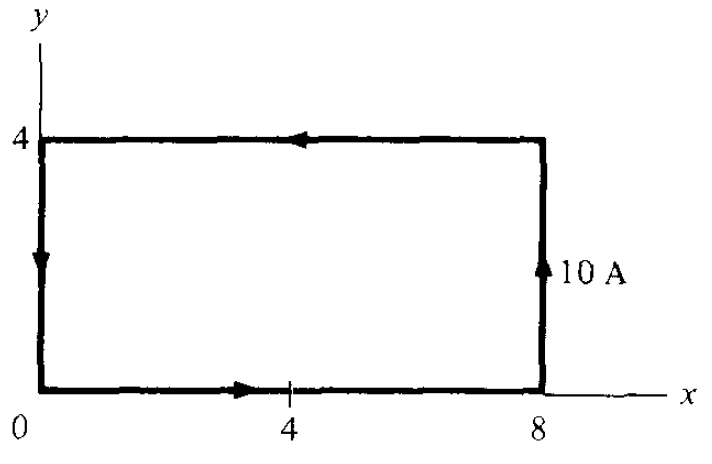
\includegraphics[scale=0.35]{Figure7-30S.png}
%\caption{Rectangular loop.}
\label{rectangular-loop}
\end{figure}
\end{document}
